
\section{Methods}


\subsection{The SaltProc modeling and simulation code}

The SaltProc tool \cite{andrei_rykhlevskii_arfc/saltproc:_201*} is designed to expand SERPENT 2
 depletion capabilities for modeling liquid-fueled \gls{MSR} for continuous reprocessing.
The Python package uses HDF5 \cite{the_hdf_group_hierarchial_1997} to store data, and the Nuclear Engineering Toolkit PyNE \cite{scopatz_pyne:_2012}
for SEPRENT output file parsing and nuclide naming. It is an open-source tool that uses a semi-continuous approach to 
simulate continuous feeds and removals in the \gls{MSR}. 

The tool structure and capabilities of SaltProc are similar to ChemTriton tool for SCALE
developed in \gls{ORNL} \cite{powers_new_2013}. SaltProc is coupled with Monte Carlo SERPENT 2
software which allows to simulate online reprocessing for irregular full-core geometry with 
high level of fidelity.  The primary function of SaltProc is to manage material streams while
SERPENT 2 performs most of the computationally heavy work, namely neutron transport and depletion
calculations. Saltproc is defined as a 
python class, where each material stream is defined as a isotopic atomic density
vector variable. This allows tracking of time-sensitive material streams such as the
Pa-233 tank in the \gls{MSBR}. The user can define the reprocessing parameters, such as the 
reprocessing interval and removal efficiency.  In addition, SaltProc provides a set of functions 
for each stream: read and write isotopic data in/from database, separate out specific isotopes 
from stream with defined efficiency, feed in specific isotopes to stream, and maintain constant 
number density of specific nuclide in the core. These attributes and functions are crucial to 
simulate the operation of a complex, multi-zone, multi-fluid \gls{MSR} and are universal for 
myriad reactor systems.

Saltproc is currently in active development in Github (https://github.com/arfc/saltproc), and has unit tests and
Travis continuous integration for sustainable development. There is also documentation
generated through Sphinx document generator for ease of use. We plan to implement
user-defined reprocessing scheme definition, two-region \gls{MSR} modeling capabilities,
and decay modeling in future releases.

Figure~\ref{fig:saltproc_flow} illustrates the  online reprocessing simulation algorithm the 
coupled SaltProc and SERPENT 2. To perform a depletion step,
SaltProc reads an external SERPENT 2 template file which is defined by the user. This file 
contains input cards with parameters such as geometry,
moderator and construction materials isotopic composition, neutron population, criticality 
cycles, total heating power, and boundary conditions.
After the depletion calculation, SaltProc reads the depleted fuel composition file (\texttt{
.bumat1}) and stores the depleted
composition isotopic vector in an HDF5 database. SaltProc only stores and edits the isotopic 
composition of the fuel stream,
which makes SaltProc a flexible tool to model any geometry: an infinite medium, a unit cell, a 
multi-zone simplified assembly, or a full core.
This flexibiliity allows the user to perform simulations of varying fidelity and computational 
intensity.

SaltProc can manage as many material streams as desired. It also may work with multiple depletion 
materials. At the end of a each depletion
step, SaltProc reads the depleted compositions and tracks each material stream individually. 
Following this, it applies chemical
separation functions to fuel stream vectors. These vectors then form a matrix (isotopics x 
timesteps) which SaltProc stores in an HDF5 database
and prints into the SERPENT 2 composition file for the next depletion calculation.

Saltproc datasets are timseries, meaning that every value is recorded every timestep. The 
datasets SaltProc produces are listed below,
where the values inside the parenthesis are the dataset sizes:

\begin{itemize}
    \item \texttt{core adensity before reproc} (number of isotopes X timesteps)
    \item \texttt{core adensity after reproc} (number of isotopes X timesteps)
    \item \texttt{Keff_BOC} (1 X timesteps)
    \item \texttt{Keff_EOC} (1 X timesteps)
    \item \texttt{Th tank adensity} (number of isotopes X timesteps)
    \item \texttt{iso codes} (number of isotopes X 1)
\end{itemize}

Liquid-fueled \gls{MSBR} design in this thesis focuses on the state of the core at an equilibrium condition, after fission products have
built up in the fuel salt during years if operation. Isotopic composition of the fuel salt continues change slightly even after decades
of operation, but the dominant nuclides that have significant impact to the neutronic behavior tend to reach an equilibrium concentration
(e.g., vary less than 1\% over several years). In contrast, from the startup of an \gls{MSBR} until the equilibrium condition,
the fuel salt composition undergoes significant changes (e.g., changes in fission products, minor actinides, and fissile
materials number density). During this period, the material feeds and removals should be optimized for the fastest \gls{MSBR} transition to an
equilibrium state. A faster transition simplifies the reactor operation because, at equilibrium, the fissile and fertile feed rates,
fission product removal rates, and corresponding core safety parameters are constant in time.

\begin{figure}[htp!] % replace 't' with 'b' to 
  \centering
  \vspace{-0.3em}
  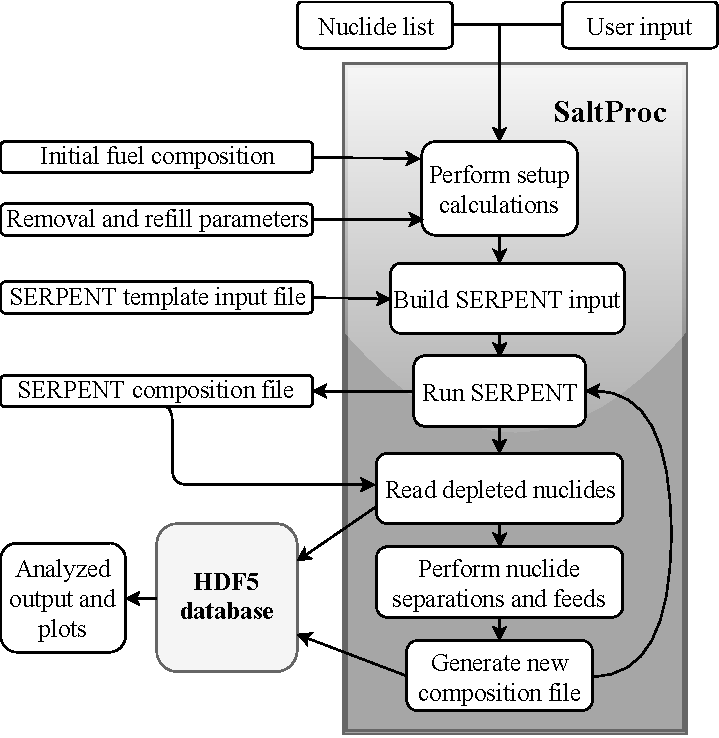
\includegraphics[width=\textwidth]{saltproc_flowchart.pdf}
  \caption{Flow chart for the Saltproc python-based tools.}
  \vspace{-1.0em}
  \label{fig:saltproc_flow}
\end{figure}
\FloatBarrier

In addition, SaltProc is able to define time-dependent material feed and removal rates to investigate the their impacts. These rates need not be
constant in SaltProc. They can be defined as piecewise functions or set to respond conditions in the core. For instance, SaltProc might increase the
fissile material feeding rate if the effective multiplication factor, $k_{eff}$, falls below a specific limit (e.g., 1.002).
These capabilities allow SaltProc to analyze fuel cycle of a generic liquid-fueled \gls{MSR}. In summary, the development approach of SaltProc focused
on producing a generic, flexible and expandable tool to give the SERPENT 2 Monte Carlo code the ability to conduct advanced in-reactor
fuel cycle analysis as well as simulate a myriad of online refueling and fuel reprocessing systems.

